\tikzstyle{num} = [rectangle, minimum width = 0.6cm, minimum height = 0.6cm, text centered,align=center,thick,draw = black,rounded corners=1.5pt]


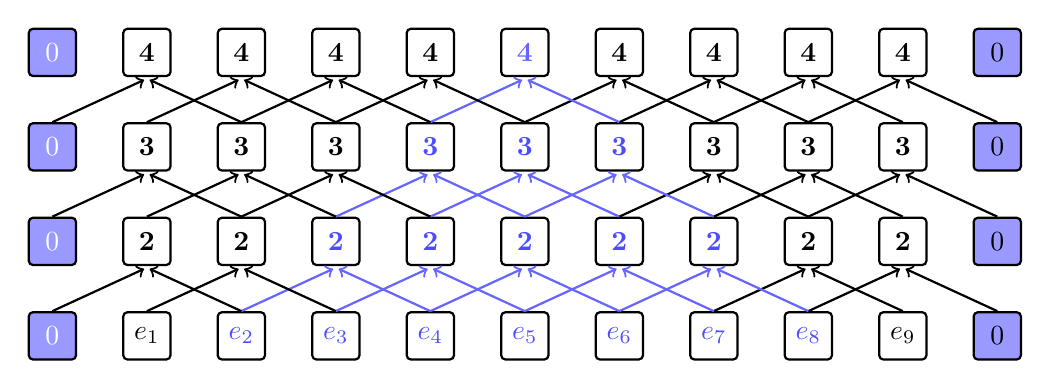
\begin{tikzpicture}[node distance = 0cm]
\node(num1_0)[num, fill = blue!40]{\textcolor{white}{$\mathbi{0}$}};
\node(num1_1)[num,right of = num1_0,xshift = 1.2cm]{$\mathbi{e}_1$};
\node(num1_2)[num,right of = num1_1,xshift = 1.2cm]{\textcolor{blue!70}{$\mathbi{e}_2$}};
\node(num1_3)[num,right of = num1_2,xshift = 1.2cm]{\textcolor{blue!70}{$\mathbi{e}_3$}};
\node(num1_4)[num,right of = num1_3,xshift = 1.2cm]{\textcolor{blue!70}{$\mathbi{e}_4$}};
\node(num1_5)[num,right of = num1_4,xshift = 1.2cm]{\textcolor{blue!70}{$\mathbi{e}_5$}};
\node(num1_6)[num,right of = num1_5,xshift = 1.2cm]{\textcolor{blue!70}{$\mathbi{e}_6$}};
\node(num1_7)[num,right of = num1_6,xshift = 1.2cm]{\textcolor{blue!70}{$\mathbi{e}_7$}};
\node(num1_8)[num,right of = num1_7,xshift = 1.2cm]{\textcolor{blue!70}{$\mathbi{e}_8$}};
\node(num1_9)[num,right of = num1_8,xshift = 1.2cm]{$\mathbi{e}_9$};
\node(num1_10)[num,right of = num1_9,xshift = 1.2cm, fill = blue!40]{$\mathbi{0}$};
%\node(A)[below of = num2,yshift = -0.6cm]{A};
%\node(B)[below of = num8,yshift = -0.6cm]{B};

\node(num2_0)[num,above of = num1_0,yshift = 1.2cm, fill = blue!40]{\textcolor{white}{$\mathbi{0}$}};
\node(num2_1)[num,right of = num2_0,xshift = 1.2cm]{\textbf2};
\node(num2_2)[num,right of = num2_1,xshift = 1.2cm]{\textbf2};
\node(num2_3)[num,right of = num2_2,xshift = 1.2cm]{\textbf{\textcolor{blue!70}2}};
\node(num2_4)[num,right of = num2_3,xshift = 1.2cm]{\textbf{\textcolor{blue!70}2}};
\node(num2_5)[num,right of = num2_4,xshift = 1.2cm]{\textbf{\textcolor{blue!70}2}};
\node(num2_6)[num,right of = num2_5,xshift = 1.2cm]{\textbf{\textcolor{blue!70}2}};
\node(num2_7)[num,right of = num2_6,xshift = 1.2cm]{\textbf{\textcolor{blue!70}2}};
\node(num2_8)[num,right of = num2_7,xshift = 1.2cm]{\textbf2};
\node(num2_9)[num,right of = num2_8,xshift = 1.2cm]{\textbf2};
\node(num2_10)[num,right of = num2_9,xshift = 1.2cm, fill = blue!40]{$\mathbi{0}$};

\node(num3_0)[num,above of = num2_0,yshift = 1.2cm, fill = blue!40]{\textcolor{white}{$\mathbi{0}$}};
\node(num3_1)[num,right of = num3_0,xshift = 1.2cm]{\textbf3};
\node(num3_2)[num,right of = num3_1,xshift = 1.2cm]{\textbf3};
\node(num3_3)[num,right of = num3_2,xshift = 1.2cm]{\textbf3};
\node(num3_4)[num,right of = num3_3,xshift = 1.2cm]{\textbf{\textcolor{blue!70}3}};
\node(num3_5)[num,right of = num3_4,xshift = 1.2cm]{\textbf{\textcolor{blue!70}3}};
\node(num3_6)[num,right of = num3_5,xshift = 1.2cm]{\textbf{\textcolor{blue!70}3}};
\node(num3_7)[num,right of = num3_6,xshift = 1.2cm]{\textbf3};
\node(num3_8)[num,right of = num3_7,xshift = 1.2cm]{\textbf3};
\node(num3_9)[num,right of = num3_8,xshift = 1.2cm]{\textbf3};
\node(num3_10)[num,right of = num3_9,xshift = 1.2cm, fill = blue!40]{$\mathbi{0}$};

\node(num4_0)[num,above of = num3_0,yshift = 1.2cm, fill = blue!40]{\textcolor{white}{$\mathbi{0}$}};
\node(num4_1)[num,right of = num4_0,xshift = 1.2cm]{\textbf4};
\node(num4_2)[num,right of = num4_1,xshift = 1.2cm]{\textbf4};
\node(num4_3)[num,right of = num4_2,xshift = 1.2cm]{\textbf4};
\node(num4_4)[num,right of = num4_3,xshift = 1.2cm]{\textbf4};
\node(num4_5)[num,right of = num4_4,xshift = 1.2cm]{\textbf{\textcolor{blue!60}4}};
\node(num4_6)[num,right of = num4_5,xshift = 1.2cm]{\textbf4};
\node(num4_7)[num,right of = num4_6,xshift = 1.2cm]{\textbf4};
\node(num4_8)[num,right of = num4_7,xshift = 1.2cm]{\textbf4};
\node(num4_9)[num,right of = num4_8,xshift = 1.2cm]{\textbf4};
\node(num4_10)[num,right of = num4_9,xshift = 1.2cm, fill = blue!40]{$\mathbi{0}$};

\draw [->, thick](num1_0.north)--([xshift=-0.1em,yshift=-0.1em]num2_1.south);
\draw [->, thick](num2_0.north)--([xshift=-0.1em,yshift=-0.1em]num3_1.south);
\draw [->, thick](num3_0.north)--([xshift=-0.1em,yshift=-0.1em]num4_1.south);
\draw [->, thick](num1_1.north)--([xshift=-0.1em,yshift=-0.1em]num2_2.south);
\draw [->, thick](num2_1.north)--([xshift=-0.1em,yshift=-0.1em]num3_2.south);
\draw [->, thick](num3_1.north)--([xshift=-0.1em,yshift=-0.1em]num4_2.south);
\draw [->, thick, color = blue!60](num1_2.north)--([xshift=-0.1em,yshift=-0.1em]num2_3.south);
\draw [->, thick](num2_2.north)--([xshift=-0.1em,yshift=-0.1em]num3_3.south);
\draw [->, thick](num3_2.north)--([xshift=-0.1em,yshift=-0.1em]num4_3.south);
\draw [->, thick, color = blue!60](num1_3.north)--([xshift=-0.1em,yshift=-0.1em]num2_4.south);
\draw [->, thick, color = blue!60](num2_3.north)--([xshift=-0.1em,yshift=-0.1em]num3_4.south);
\draw [->, thick](num3_3.north)--([xshift=-0.1em,yshift=-0.1em]num4_4.south);
\draw [->, thick, color = blue!60](num1_4.north)--([xshift=-0.1em,yshift=-0.1em]num2_5.south);
\draw [->, thick, color = blue!60](num2_4.north)--([xshift=-0.1em,yshift=-0.1em]num3_5.south);
\draw [->, thick, color = blue!60](num3_4.north)--([xshift=-0.1em,yshift=-0.1em]num4_5.south);
\draw [->, thick, color = blue!60](num1_5.north)--([xshift=-0.1em,yshift=-0.1em]num2_6.south);
\draw [->, thick, color = blue!60](num2_5.north)--([xshift=-0.1em,yshift=-0.1em]num3_6.south);
\draw [->, thick](num3_5.north)--([xshift=-0.1em,yshift=-0.1em]num4_6.south);
\draw [->, thick, color = blue!60](num1_6.north)--([xshift=-0.1em,yshift=-0.1em]num2_7.south);
\draw [->, thick](num2_6.north)--([xshift=-0.1em,yshift=-0.1em]num3_7.south);
\draw [->, thick](num3_6.north)--([xshift=-0.1em,yshift=-0.1em]num4_7.south);
\draw [->, thick](num1_7.north)--([xshift=-0.1em,yshift=-0.1em]num2_8.south);
\draw [->, thick](num2_7.north)--([xshift=-0.1em,yshift=-0.1em]num3_8.south);
\draw [->, thick](num3_7.north)--([xshift=-0.1em,yshift=-0.1em]num4_8.south);
\draw [->, thick](num1_8.north)--([xshift=-0.1em,yshift=-0.1em]num2_9.south);
\draw [->, thick](num2_8.north)--([xshift=-0.1em,yshift=-0.1em]num3_9.south);
\draw [->, thick](num3_8.north)--([xshift=-0.1em,yshift=-0.1em]num4_9.south);

\draw [->, thick](num1_2.north)--([xshift=0.1em,yshift=-0.1em]num2_1.south);
\draw [->, thick](num2_2.north)--([xshift=0.1em,yshift=-0.1em]num3_1.south);
\draw [->, thick](num3_2.north)--([xshift=0.1em,yshift=-0.1em]num4_1.south);
\draw [->, thick](num1_3.north)--([xshift=0.1em,yshift=-0.1em]num2_2.south);
\draw [->, thick](num2_3.north)--([xshift=0.1em,yshift=-0.1em]num3_2.south);
\draw [->, thick](num3_3.north)--([xshift=0.1em,yshift=-0.1em]num4_2.south);
\draw [->, thick, color = blue!60](num1_4.north)--([xshift=0.1em,yshift=-0.1em]num2_3.south);
\draw [->, thick](num2_4.north)--([xshift=0.1em,yshift=-0.1em]num3_3.south);
\draw [->, thick](num3_4.north)--([xshift=0.1em,yshift=-0.1em]num4_3.south);
\draw [->, thick, color = blue!60](num1_5.north)--([xshift=0.1em,yshift=-0.1em]num2_4.south);
\draw [->, thick, color = blue!60](num2_5.north)--([xshift=0.1em,yshift=-0.1em]num3_4.south);
\draw [->, thick](num3_5.north)--([xshift=0.1em,yshift=-0.1em]num4_4.south);
\draw [->, thick, color = blue!60](num1_6.north)--([xshift=0.1em,yshift=-0.1em]num2_5.south);
\draw [->, thick, color = blue!60](num2_6.north)--([xshift=0.1em,yshift=-0.1em]num3_5.south);
\draw [->, thick, color = blue!60](num3_6.north)--([xshift=0.1em,yshift=-0.1em]num4_5.south);
\draw [->, thick, color = blue!60](num1_7.north)--([xshift=0.1em,yshift=-0.1em]num2_6.south);
\draw [->, thick, color = blue!60](num2_7.north)--([xshift=0.1em,yshift=-0.1em]num3_6.south);
\draw [->, thick](num3_7.north)--([xshift=0.1em,yshift=-0.1em]num4_6.south);
\draw [->, thick, color = blue!60](num1_8.north)--([xshift=0.1em,yshift=-0.1em]num2_7.south);
\draw [->, thick](num2_8.north)--([xshift=0.1em,yshift=-0.1em]num3_7.south);
\draw [->, thick](num3_8.north)--([xshift=0.1em,yshift=-0.1em]num4_7.south);
\draw [->, thick](num1_9.north)--([xshift=0.1em,yshift=-0.1em]num2_8.south);
\draw [->, thick](num2_9.north)--([xshift=0.1em,yshift=-0.1em]num3_8.south);
\draw [->, thick](num3_9.north)--([xshift=0.1em,yshift=-0.1em]num4_8.south);
\draw [->, thick](num1_10.north)--([xshift=0.1em,yshift=-0.1em]num2_9.south);
\draw [->, thick](num2_10.north)--([xshift=0.1em,yshift=-0.1em]num3_9.south);
\draw [->, thick](num3_10.north)--([xshift=0.1em,yshift=-0.1em]num4_9.south);
\end{tikzpicture}